\section{Results and Discussion}

\begin{figure}[H]
	\centering
	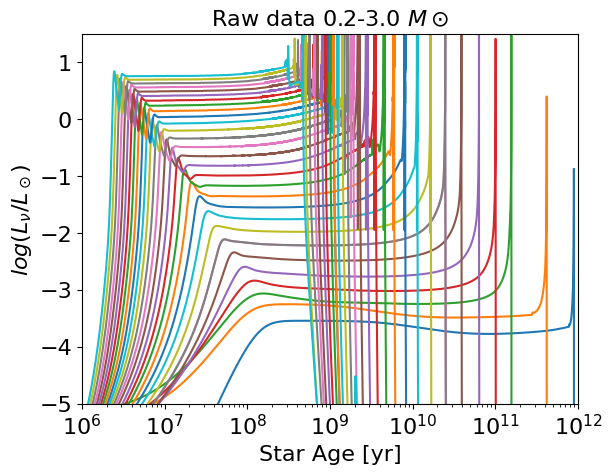
\includegraphics[width=\textwidth]{assets/raw.png}
	\caption{Raw data $0.2-3.0 M\odot$.}
	\label{fig:raw}
\end{figure}

\begin{figure}[H]
	\centering
	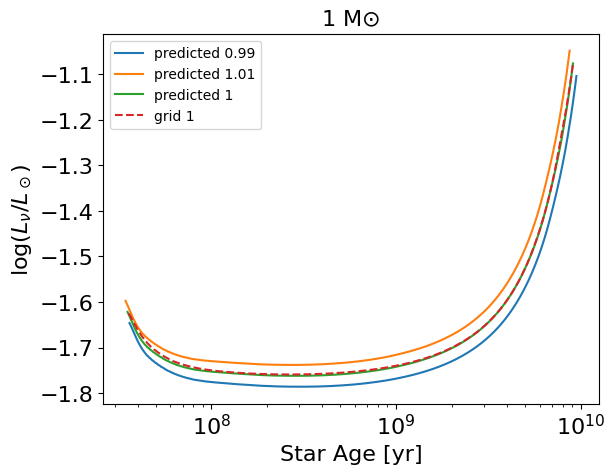
\includegraphics[width=\textwidth]{assets/output1.png}
	\caption{Sun $1M\odot$ Testing Data.}
	\label{fig:SunTest}
\end{figure}

\begin{table}[H]
    \centering
	\caption{Stars with their mass and distance.}
	\label{tab:stars and mass}
	\begin{tabular}{ccc}
		\toprule
		Star & Mass [$M\odot$]  & Distance [$pc$] \\
		\midrule
		$\tau$ ceti & $0.78$ & $3.65$\\
		Sun & $1$ & $4.85\times 10^{-6}$\\
		\bottomrule
	\end{tabular}
\end{table}

\begin{figure}[H]
	\centering
	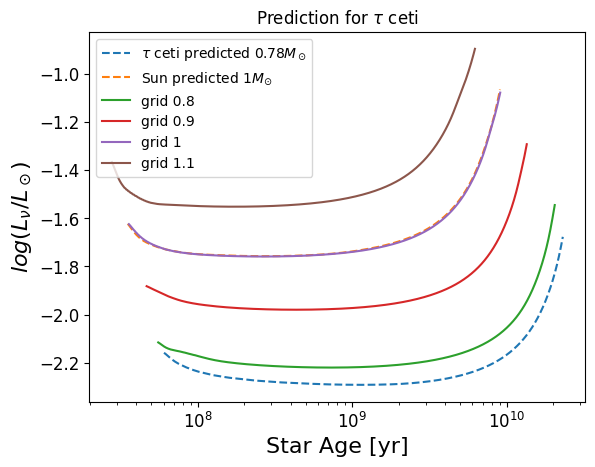
\includegraphics[width=\textwidth]{assets/predtauceti.png}
	\caption{Prediction for $\tau$ ceti $0.78 M\odot$.}
	\label{fig:tau}
\end{figure}

\begin{figure}[H]
	\centering
	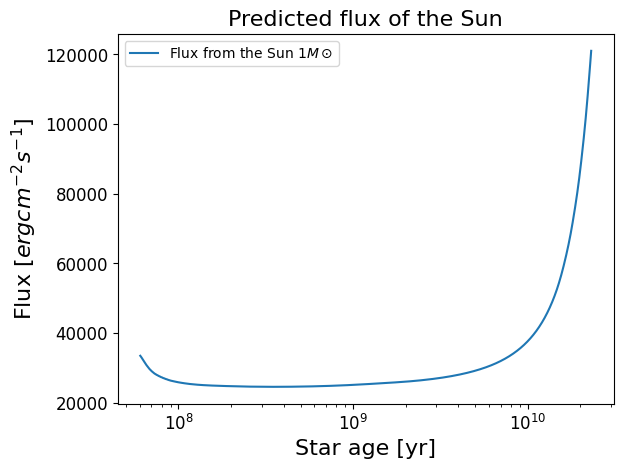
\includegraphics[width=\textwidth]{assets/fluxsun.png}
	\caption{Prediction for Flux of Sun $1 M\odot$.}
	\label{fig:fluxsun}
\end{figure}

\begin{figure}[H]
	\centering
	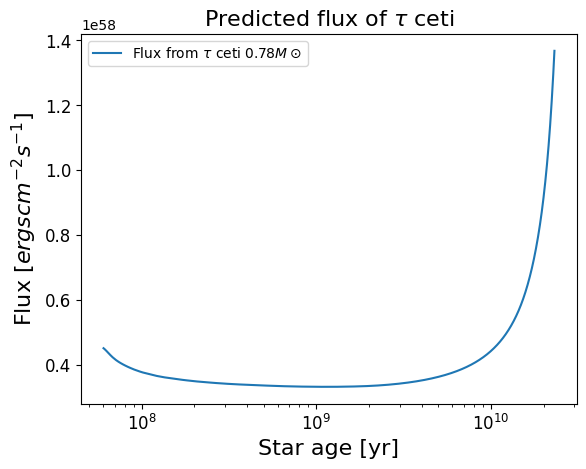
\includegraphics[width=\textwidth]{assets/fluxtau.png}
	\caption{Prediction for flux of $\tau$ ceti $0.78 M\odot$.}
	\label{fig:fluxtau}
\end{figure}

\begin{figure}[H]
	\centering
	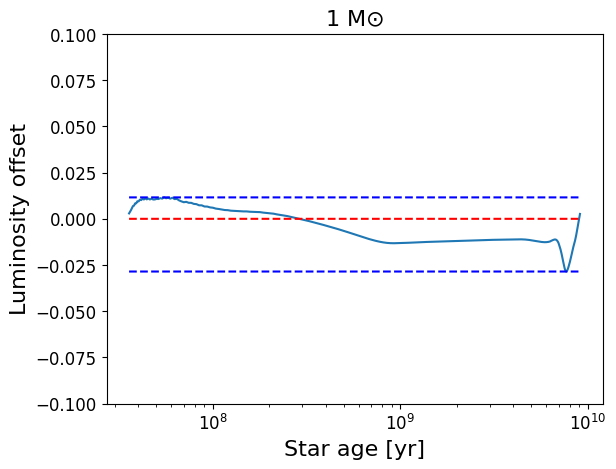
\includegraphics[width=\textwidth]{assets/error 1.png}
	\caption{Luminosity Offset for $1M\odot$.}
	\label{fig:error1}
\end{figure}
\begin{figure}[H]
	\centering
	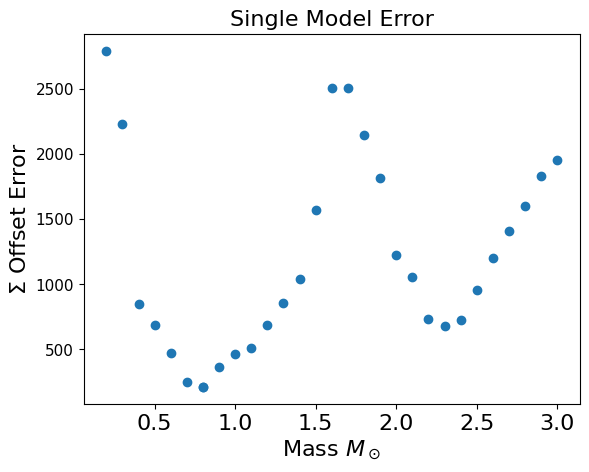
\includegraphics[width=\textwidth]{assets/singlemodeerror.png}
	\caption{Single Model Error.}
	\label{fig:errorsingle}
\end{figure}

\begin{figure}[H]
	\centering
	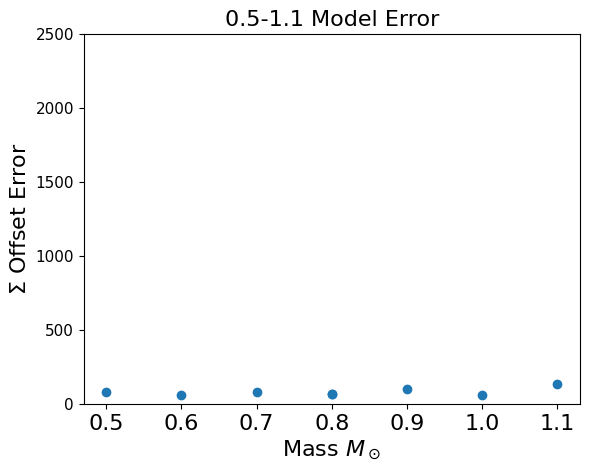
\includegraphics[width=\textwidth]{assets/0.5-1.1Error.png}
	\caption{$0.5-2.2M\odot$ Model Error.}
	\label{fig:error0.5-1.1}
\end{figure}